%  ========================================================================
%  Copyright (c) 1985-2014 The University of Washington
%
%  Licensed under the Apache License, Version 2.0 (the "License");
%  you may not use this file except in compliance with the License.
%  You may obtain a copy of the License at
%
%      http://www.apache.org/licenses/LICENSE-2.0
%
%  Unless required by applicable law or agreed to in writing, software
%  distributed under the License is distributed on an "AS IS" BASIS,
%  WITHOUT WARRANTIES OR CONDITIONS OF ANY KIND, either express or implied.
%  See the License for the specific language governing permissions and
%  limitations under the License.
%  ========================================================================
%

% Documentation for University of Washington thesis LaTeX document class
% by Jim Fox
% fox@washington.edu
%
%    Revised for version 2015/03/03 of uwthesis.cls
%
%    This document is contained in a single file ONLY because
%    I wanted to be able to distribute it easily.  A real thesis ought
%    to be contained on many files (e.g., one for each chapter, at least).
%
%    To help you identify the files and sections in this large file
%    I use the string '==========' to identify new files.
%
%    To help you ignore the unusual things I do with this sample document
%    I try to use the notation
%       
%    % --- sample stuff only -----
%    special stuff for my document, but you don't need it in your thesis
%    % --- end-of-sample-stuff ---


%    Printed in twoside style now that that's allowed
%
 
\documentclass [11pt, proquest] {/Users/jgruszko/Documents/Thesis/Template/uwthesis}[2015/03/03]

\usepackage{graphicx}
 \usepackage{caption}
 \usepackage{subcaption}
 \captionsetup{compatibility=false}
%
% The following line would print the thesis in a postscript font 

% \usepackage{natbib}
% \def\bibpreamble{\protect\addcontentsline{toc}{chapter}{Bibliography}}

\setcounter{tocdepth}{1}  % Print the chapter and sections to the toc
 

% ==========   Local defs and mods
%
% ==========   Local defs and mods
%

% --- sample stuff only -----
% These format the sample code in this document

\usepackage{alltt}  % 
\newenvironment{demo}
  {\begin{alltt}\leftskip3em
     \def\\{\ttfamily\char`\\}%
     \def\{{\ttfamily\char`\{}%
     \def\}{\ttfamily\char`\}}}
  {\end{alltt}}
 
  % Definitions and macros
\newcommand{\degrees}{$^{\circ}$}                                         % makes a correct degree symbol
\newcommand{\cpp}{C\protect\raisebox{.25ex}{++}\ }               % formats C++ correctly
\newcommand{\MJ}{M{\footnotesize AJORANA}}                        % this works for bolding in titles and the toc
\newcommand{\MJDemo}{D{\footnotesize EMON\-STRAT\-OR}} 	% this works for bolding in titles and the toc
\newcommand{\snop}{SNO\protect\raisebox{.25ex}{+}}             % formats SNO+ nicely
\newcommand{\nonubb}  {${0 \nu \beta \beta}$}                       % neutrinoless double beta decay in math mode
\newcommand{\iso}[2]{$^{#1}$#2}                                        % Makes a properly formatted isotope symbol e.g. \iso{28}{Si}

% metafont font.  If logo not available, use the second form
%
% \font\mffont=logosl10 scaled\magstep1
\let\mffont=\sf
% --- end-of-sample-stuff ---
  



\begin{document}
 
% ==========   Preliminary pages
\prelimpages
 
%
% ----- copyright and title pages
%
\Title{Surface Alpha Interactions in P-Type Point-Contact HPGe Detectors: Maximizing Sensitivity of $^{76}$Ge Neutrinoless Double-Beta Decay Searches}
\Author{Julieta Gruszko}
\Year{2017}
\Program{UW Physics}

\Chair{Jason Detwiler}{Assistant Professor}{Physics}
\Signature{Ann Nelson}
\Signature{Grey Rybka}

\copyrightpage

 \titlepage  

%
% ----- signature and quoteslip are gone
%

%
% ----- abstract
%


\setcounter{page}{-1}
\abstract{
Though the existence of neutrino oscillations proves that neutrinos must have non-zero mass, Beyond-the-Standard-Model physics is needed to explain the origins of that mass. One intriguing possibility is that neutrinos are Majorana particles, i.e., they are their own anti-particles. Such a mechanism could naturally explain the observed smallness of the neutrino masses, and would have consequences that go far beyond neutrino physics, with implications for Grand Unification and leptogenesis. 

If neutrinos are Majorana particles, they could undergo neutrinoless double-beta decay (\nonubb), a hypothesized rare decay in which two antineutrinos annihilate one another. This process, if it exists, would be exceedingly rare, with a half-life over $10^{25}$ years. Therefore, searching for it requires experiments with extremely low background rates. One promising technique in the search for \nonubb\ is the use of P-type point-contact (\ppc) high-purity Germanium (HPGe) detectors enriched in $^{76}$Ge, operated in large low-background arrays. This approach is used, with some key differences, by the \MJ\ and GERDA Collaborations. 

A problematic background in such large granular detector arrays is posed by alpha particles incident on the surfaces of the detectors, often caused by $^{222}$Rn contamination of parts or of the detectors themselves. In the \textsc{Majorana Demonstrator}, events have been observed that are consistent with energy-degraded alphas originating near the passivated surface of the detectors, leading to a potential background contribution in the region-of-interest for neutrinoless double-beta decay. However, it is also observed that when energy deposition occurs very close to the passivated surface, high charge trapping occurs along with subsequent slow charge re-release. This leads to both a reduced prompt signal and a measurable change in slope of the tail of a recorded pulse. Here we discuss the characteristics of these events and the development of a filter that can identify the occurrence of this delayed charge recovery (DCR) effect, allowing for the efficient rejection of passivated surface alpha events in analysis. 

Using a dedicated test-stand called the TUM Upside-down BEGe (TUBE) scanner, we have characterized the response of a \ppc\ detector like those used in the \DEM\ to alphas incident on the sensitive surfaces, developing a model for the radial dependence of the energy loss to charge trapping and determining the dominant mechanism behind the delayed charge effect. We have also used these measurements to demonstrate the complementarity of the DCR analysis with the drift-time analysis that is used to identify alpha background candidate events in the GERDA detectors. Using these two methods, we demonstrate the ability to effectively reject all alpha events (to within statistical uncertainty) with only 0.2\% bulk event sacrifice. 

Applying the DCR analysis to the events observed in the \MJ\ \DEM, we find that it reduces the backgrounds in the \nonubb\ region-of-interest by a factor of 31, increasing the expected experimental sensitivity by a factor of 3 over the lifetime of the \DEM. The results of the dedicated measurements in the TUBE scanner can be used to build a background model for alpha decays in the \DEM ; here, we examine two simplified geometric models for the alpha source distribution and find that the observed spectral shape is consistent with alpha events originating in the plastics of the detector units. 
 }
%
% ----- contents & etc.
%
\tableofcontents
\listoffigures
\listoftables  % I have no tables
 
%
% ----- glossary 
%
\chapter*{Glossary}      % starred form omits the `chapter x'
\addcontentsline{toc}{chapter}{Glossary}
\thispagestyle{plain}
%
\begin{glossary}
\item[MJD] The \MJ\ \MJDemo\ 
\item[HPGe] High-purity Germanium
\item[PPC] P-type point contact detector.
\end{glossary}

% ==========      Text pages
%

\textpages
 
% ========== Chapter 1
% ========== Chapter 1
 
\chapter {Neutrino Physics and \nonubb Introduction}
\section{Neutrinos as a Key to New Physics}
\subsection{The ``Desperate Remedy"}
Since its introduction by Wolfgang Pauli in 1930, the neutrino has been allowing physicists to reconcile theories and experiments that did not quite align. At the time, the theories in question were the conservation of energy and angular momentum; beta decay observations seemed to violate these key principles. Instead of carrying away the full Q-value of the decay, the observed electrons could carry off a range of energies up to that value. And instead of going off back-to-back, as expected in a two-body decay under momentum conservation laws, the recoiling nucleus and electron could have any angle between them. 

As a ``desperate remedy," Pauli proposed the neutrino \cite{Pauli1930}-- a light, neutral particle that was being created in the decay, carrying off the missing energy and momentum. If it did not interact via the strong or electromagnetic forces, such a particle would easily escape most detectors. In fact, the elusive neutrino escaped detection for over twenty years, until it was eventually observed in 1956 \cite{Cowan1956}. With the addition of this particle to the standard model, beta decay was explained as a three-body process, and the conservation laws were saved.

\subsection{The Solar Neutrino Problem}
Along with the neutrino, the concepts of lepton number and lepton number conservation were introduced. This value, in the standard model, is conserved in weak interactions, which proceed via two classes of vertex, called the neutral and charged currents. The Feynman diagrams for these processes are seen in Fig.~\ref{weak_diagrams}. In the charged current interactions, a charged lepton (i.e. the electron, muon, or tau, or their antiparticles) participates in the interaction, and the (anti-)neutrino always occurs with the W+(-) boson. In the neutral current interaction, a lepton and its corresponding anti-lepton always participate along with the Z boson. 

\begin{figure}[h]
\hfil 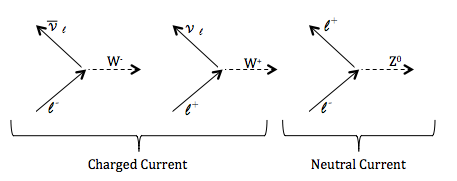
\includegraphics[width = .80\textwidth]{/Users/jgruszko/Documents/Thesis/Images/Ch1/WeakDiagrams.png} \hfil
\caption{The primitive vertices of the Feynman diagrams for weak interactions between leptons in the standard model. Equivalent vertices exist for the quarks. \cite{PDG2014}}
\label{weak_diagrams}
\end{figure}

There are (at least) three neutrino flavors, corresponding to the three charged leptons, which form a basis of flavor eigenstates. They are created in these eigenstates-- in a charged current interaction emitting an electron, for instance, the standard model requires that an electron anti-neutrino is also created. Originally, it was believed that neutrinos also followed lepton-flavor conservation. Since in the standard model, neutrinos are massless, that electron anti-neutrino would propagate in its flavor eigenstate, and remain an electron anti-neutrino. 

With this assumption firmly in place, physicists began to attempt to detect the neutrinos created in the sun. Based on astrophysical models of solar fusion processes \cite{Bahcall}, 7E10 $\nu_{e}$/cm$^2$/s were expected to reach earth. When Ray Davis measured the solar neutrino flux in the Homestake experiment, however, he found far fewer $\nu_{e}$, about a third the flux that Bahcall's model predicted. Later experiments confirmed this low $\nu_{e}$ flux -- once again the theory (this time the theory behind fusion models of the sun) and the experiments did not agree.

As in the 1930s, the unexpected physics of the neutrino `saved the day.' If the neutrino was not massless, as the Standard Model seemed to assert, but instead had a small mass, it would not propagate in its flavor eigenstate. Instead it would propagate in a mass eigenstate, and if these eigenstates were not equivalent, it would change from one flavor to another as it traveled from the sun to detectors on earth. 

Testing this theory required detectors that could measure the total neutrino flux, instead of just the flux of electron-flavor neutrinos. With the construction of Super-Kamiokande and SNO, the total neutrino flux was measured in 2001, and neutrino oscillations were seen. The mixing of the mass eigenstates in a given flavor eigenstate is described by the PMNS matrix, 
\[
\begin{bmatrix}
\nu_e\\
\nu_\mu\\
\nu_\tau\\
\end{bmatrix}
=
\begin{bmatrix}
U_{e1} & U_{e2} & U_{e3} \\ 
U_{\mu1} & U_{\mu2} & U_{\mu3} \\ 
U_{\tau1} & U_{\mu2} & U_{\mu3} \\ 
\end{bmatrix}
\begin{bmatrix}
\nu_1\\
\nu_2\\
\nu_3\\
\end{bmatrix}
\]

Unlike the quarks, neutrino

- Focus on oscillation, expand this paragraph:
As the properties of neutrinos become better understood, they continue to play this role, pulling our theories back from the brink of incorrectness-- the ``solar neutrino problem" was eventually resolved by the introduction of neutrino flavor oscillations and neutrino mass. \cite{PDG2014} Other proposed aspects of neutrino physics could reveal neutrinoless double beta decay, a lepton number-violating process that could explain the source of matter/anti-matter imbalance in the universe. If this decay were observed, the neutrino would be a Majorana particle (meaning that it is its own antiparticle), explaining the origin and smallness of the neutrino masses.

\subsection{Role of neutrinos in the standard model} 
The neutrinos are standard-model fermions that interact only via gravity and the weak force. 

The weak interaction 


Neutrino oscillation arises because the neutrinos have mass eigenstates (called 1, 2, and 3) that are different from their flavor eigenstates. Therefore, as they propagate in mass/momentum eigenstates, their flavors change according to the PMNS mixing matrix, a unitary matrix that connects the two bases.  The differences in the masses squared of the states also appears in the oscillation probabilities, so these values can be found from neutrino oscillation experiments. The sign of m$_{2,3}$$^{2}$, however, is currently unknown, leading to what are called the ``normal" and ``inverted" cases of the neutrino mass hierarchy, as seen in Fig.~\ref{mass_hierarchy}. 

\begin{figure}[]
\hfil 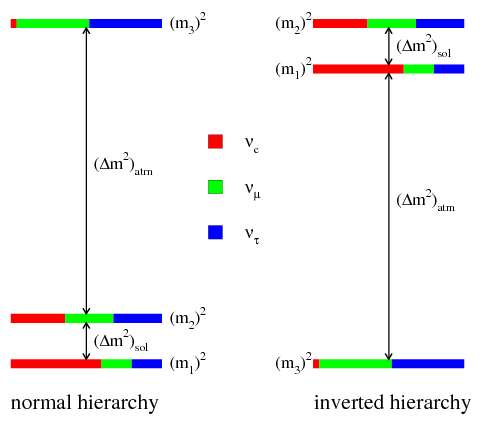
\includegraphics[width = .40\textwidth]{/Users/jgruszko/Documents/Thesis/Images/Ch1/MassHierarchy.png} \hfil
\caption{The two possible cases of the neutrino mass hierarchy \cite{Hewett2012}}
\label{mass_hierarchy}
\end{figure}

	- chirality, helicity, weyl spinors, 
\subsection{Mass mechanisms (Dirac and Majorana)} 
	- why both are problematic
\subsection{Outstanding problems in neutrino physics}
	- Unknown SM neutrino properties (mass, mass hierarchy), sterile neutrinos
         - Neutrino mass-scale problem

Additionally, the overall neutrino mass is not known. The lowest limits, derived from the shape of the $^{3}$He $\beta$-decay spectrum, give $m_{\bar{\nu}_{e}} < 2.3~eV$ \cite{Eitel2005}. More stringent limits, below $0.23~eV$, have been derived from cosmic microwave background observations \cite{PlanckXVI_2013}, but these values are highly model-dependent. The KATRIN experiment plans to directly probe masses down to $m_{\bar{\nu}_{e}} \sim 0.20~eV$ \cite{KATRIN2015}

\subsection{The Neutrino- Majorana or Dirac?}
Because neutrino oscillations have been observed, it is clear that neutrinos have non-zero mass. Minimalistic Higgs models, however, require fine-tuning, unnaturally leaving the neutrino mass about six orders of magnitude smaller than the masses of the other standard model particles. Any mechanism for neutrino mass that avoids this unnaturalness must come from an extension to the standard model. One possibility, called the ``see-saw mechanism," relies on the addition of a Majorana mass term \cite{Supergravity1979}. With the introduction of this term, there are no longer (non-interacting) right-handed neutrinos and left-handed antineutrinos. Instead, the neutrino and antineutrino are opposite-helicity states of the same Majorana particle. The Majorana mass term would contribute to the overall observed neutrino mass along with remaining Dirac mass terms, and could lead to lepton-number violating interactions. These interactions also allow a mechanism by which baryogenesis could be possible, leading to matter/anti-matter imbalance in the observable universe. \cite{DiBari2012}  


	- Nature of neutrino mass
	- Matter asymm, Seesaw mechanism

\section{Double beta-decay introduction}
\subsection{2nBB}
- 0nBB
	
\subsection{Neutrinoless Double Beta Decay}
The most promising process by which to discover the nature of the neutrino is neutrinoless double beta decay. In standard-model two neutrino double-beta decay, a nucleus that contains an even number of nucleons is energetically forbidden from decaying via single beta-decay. Instead, two beta decays occur, leading to the emission of two electrons and two electron anti-neutrinos. In the neutrinoless version of this process the anti-neutrino is exchanged as a virtual particle-- it functions as an outgoing antineutrino for one of the beta decays, and as an incoming neutrino for the other decay. Thus, no neutrinos are seen in the final state:
$$M(A, Z) \rightarrow D(A, Z+2) + 2 e^{-},$$
 and all of the energy of the decay is carried by the electrons. Due to momentum conservation, the nucleons carry a negligible amount of the energy. This decay relies on the non-conservation of lepton number, which is allowed in the Standard Model, though it has not yet been observed, on the Majorana nature of the neutrino, and on the fact that the neutrino is in a mixed helicity state. Because of the last consideration, the effective size of the Majorana mass term, 
 $$\langle m_{\beta\beta} \rangle = |\sum\limits_{i=1}^3 U^2_{ei}m_i|,$$
 where $U_{ei}$ is the mixture of neutrino mass eigenstates $i$ in the electron neutrino, appears in the $0\nu\beta\beta$ rate:
 $$(T_{1/2}^{0\nu})^{-1} = G^{0\nu}|M_{0\nu}|^{2}\left(\frac{\langle m_{\beta\beta} \rangle}{m_e}\right)^2 .$$
 $G^{0\nu}$ is a phase space factor, $M_{0\nu}$ is the nuclear matrix element, and $m_e$ is the electron mass. Because they contribute to $m_{\beta\beta}$, both the overall neutrino mass and the mass hierarchy can contribute to the observed rate, as seen in Fig.~\ref{0nBBrate}. The experimental signature of such a decay would be a delta-peak in energy at the endpoint of the two-neutrino mode spectrum, as in Fig.~\ref{0nBBspectrum}.
 
 \begin{figure}[h]
 \centering
    \begin{subfigure}[b]{.40\textwidth}
      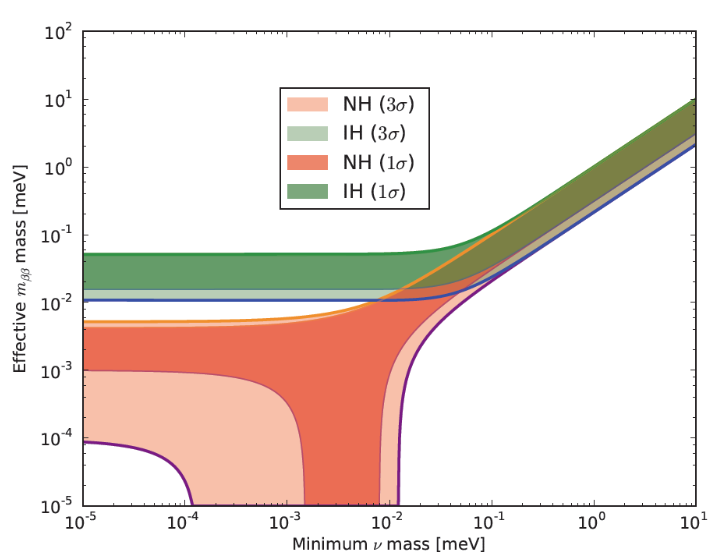
\includegraphics[width =\textwidth]{/Users/jgruszko/Documents/Thesis/Plots/Ch1/0nBB_Rate.png}
       \caption{$m_{\beta\beta}$, and therefore the $0\nu\beta\beta$ rate, depend on the neutrino mass hierarchy and the overall mass scale \cite{ZuberINT2015} .}
        \label{0nBBrate}
        \end{subfigure}   
         \hfil
        \begin{subfigure}[b]{0.4\textwidth}
      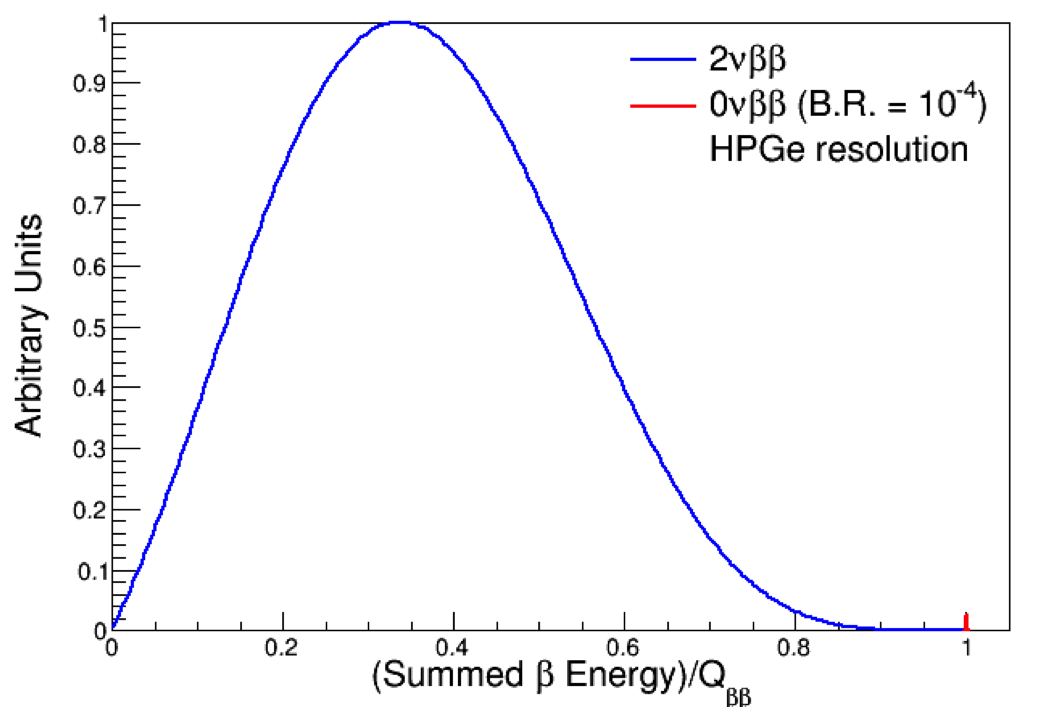
\includegraphics[width =\textwidth]{/Users/jgruszko/Documents/Thesis/Plots/Ch1/DoubleBetaEnergy.png} 
      \caption{The experimental signature of $0\nu\beta\beta$ decay as it would appear in \iso{76}{Ge}. Plot courtesy of Jason Detwiler.}
      \label{0nBBspectrum}
    \end{subfigure}   
\end{figure}
 

	- Neutrino mass dependence
- Potential implications of 0nBB
\section{Measuring \nonubb}
- Experimental requirements
\subsubsection{Observing 0$\nu\beta\beta$}
Current limits set the $0\nu\beta\beta$ half-life to greater than $10^{25}$ years \cite{EXO2014}. To observe such a rare decay, backgrounds of $0\nu\beta\beta$ experiments must be extremely low, and the mass of source material must be as large as possible. Several strategies are commonly used by the $0\nu\beta\beta$ community. 

Some are determined solely by the choice of source material:
\begin{itemize}
\item Choice of Q Value: The higher the Q-value of the $0\nu\beta\beta$ decay in some material, the less background contamination will occur in the signal region. While incomplete energy collection, Compton scattering, and other processes can cause background events to appear at energies below the peak value of the decay, events generally cannot gain energy by any process. 
\item Enrichment: Source materials often have to be enriched in the $0\nu\beta\beta$ isotope to allow for higher source masses without increasing backgrounds. The ease and expense of this process varies widely depending on the material, as does the need for enrichment.
\item Favorable Matrix Elements: $M_{0\nu}$ varies between isotopes; a favorable rate could increase the $0\nu\beta\beta$ rate. However, different calculation strategies lead to variation in these values that is on the order of the difference between isotopes. See \cite{Simkovic2009} for further discussion. 
\item Low $2\nu\beta\beta$ Rate: The resolution of any detector is imperfect, so events from the high-energy tail of the $2\nu\beta\beta$ will contribute to the background. The $2\nu$ rate is unrelated to the $0\nu$ rate.
\end{itemize} 
Unfortunately, there is no ``magic bullet" isotope for $0\nu\beta\beta$ that has all the favorable properties. 

Other strategies for background reduction are affected by the detector technology used and the design of the experiment:
\begin{itemize}
\item Source as Detector: Using the same material for both source and detector increases efficiency and makes it easier to increase source mass without increasing backgrounds.
\item Surface Event Rejection and Fiducial Volume Cuts: Generally, the bulk of the source/detector material is low in background, and most background events are from surface contamination, external sources or other components of the experiment. Detection strategies that allow surface events to be removed from the data set can often reduce backgrounds by taking advantage of self-shielding.
\item Multi-Site Rejection and Particle Identification: Many backgrounds are from $\gamma$ and $\alpha$ particles. The former often lead to multi-site interactions, while $0\nu\beta\beta$ is by its nature a single-site process, since electrons have much a shorter mean-free-path than photons in detector materials. If the detector can distinguish between multi-site and single-site interactions, backgrounds can be reduced. $\alpha$ backgrounds can be distinguished from $e/\gamma$ interactions in many two-energy-channel detectors, like time projection chambers and scintillating bolometers, and similarly reduced. 
\item High Resolution: Higher resolution makes background events easier to identify and shrinks the region of interest (ROI) for $0\nu\beta\beta$ decay, making background requirements less stringent.
\item Low Thresholds: Low energy thresholds are not required, but can allow better identification of high-energy backgrounds through timing cuts that search for L- and K-shell decay peaks of short-lived intermediate states of certain background decays. 
\item Large Overburden: All competitive $0\nu\beta\beta$ decay experiments are housed underground, to decrease the rate of cosmic-ray backgrounds and cosmogenic activation of detector materials. 
\end{itemize}


	- Advantages of 76Ge
- Backgrounds and sensitivity
- Status of the field
	- Past experiments
A controversial claim of observed $0\nu\beta\beta$ in \iso{76}{Ge} was published by Klapdor-Kleingrothaus et. al \cite{KK2001} in 2001. The current generation of experiments aims to evaluate this claim at high confidence and evaluate techniques for future experiments. The goal of the next generation of experiments is to search the entire inverted-hierarchy region, which requires 1 tonne of source material, given reasonably achievable backgrounds. See Fig.~\ref{IH_Discovery}. 

\begin{figure}[h]
\hfil 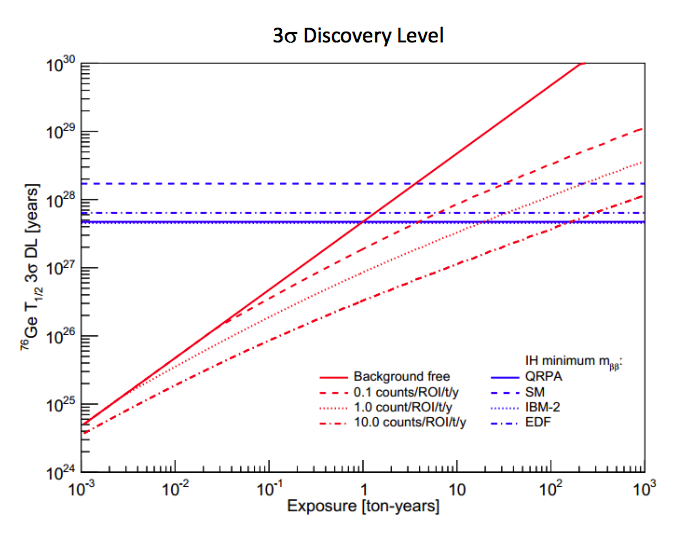
\includegraphics[width = .60\textwidth]{/Users/jgruszko/Documents/Thesis/Plots/Ch1/IH_Discovery.png} \hfil
\caption{The background requirements and exposure needed for $3\sigma$ discovery-level observation of $0\nu\beta\beta$ decay, assuming the inverted hierarchy. Plot courtesy of Jason Detwiler.}
\label{IH_Discovery}
\end{figure}

	- Gerda
\section{The \MJDemo}
\subsection{The \MJ~\MJDemo}
The \MJ~\MJDemo, the $0\nu\beta\beta$ decay search that is the focus of much of this thesis, is an experiment made up of 40 kg of PPC detectors. 30 kg of this mass is enriched to 87\% \iso{76}{Ge}, the double-beta decay parent isotope, and 10 kg is in natural-abundance detectors. The \MJDemo~uses a staged, modular approach to construction, making its techniques naturally scalable to a tonne-scale experiment. 

The largest advantage of PPCs for $0\nu\beta\beta$ decay searches is in their pulse shape characteristics. Unlike in coaxial detectors, the distance that must be traveled by a charge cloud varies depending on where in the detector it is produced, as is clear in Fig.~\ref{PPCField}. Therefore, multi-site events, in which a $\gamma$ ray deposits energy at multiple points in the crystal, have longer rise times for a given energy, and can be cut to reduce backgrounds. 

\begin{figure}[h]
\hfil 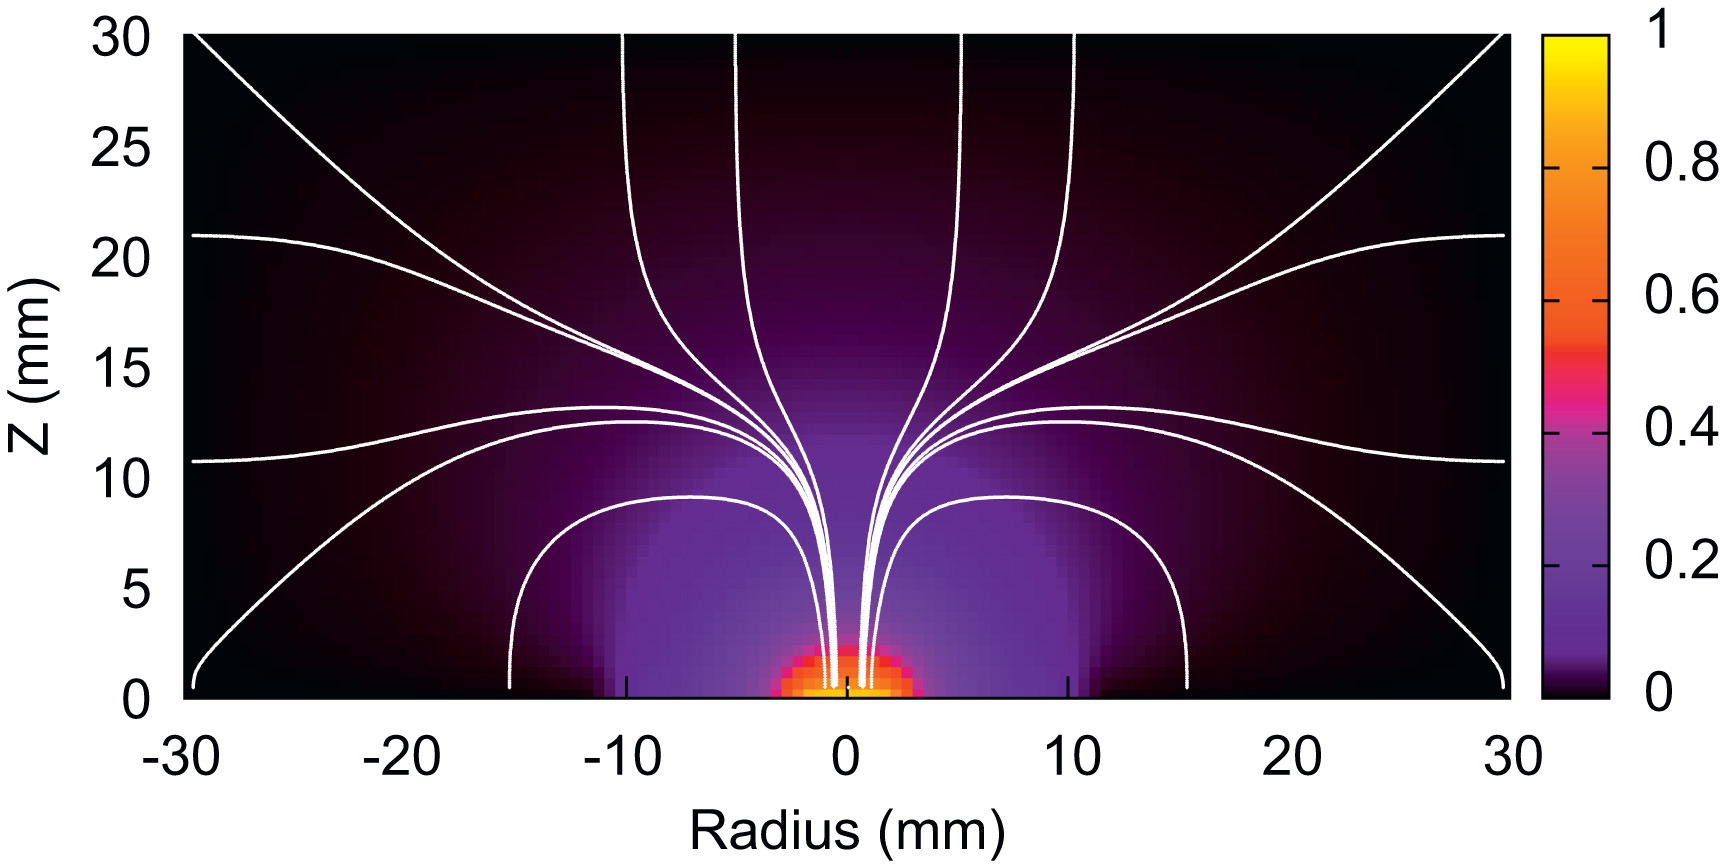
\includegraphics[width = .60\textwidth]{/Users/jgruszko/Documents/Thesis/Images/Ch1/PPCField.jpg} \hfil
\caption{A simulation of the weighting potential inside a PPC shows that charge drift paths (in white) are long and highly position-dependent. \cite{Aalseth2011}}
\label{PPCField}
\end{figure}

	- LEGeND


 
%
% ==========   Bibliography
%

\bibliographystyle{plain}
\bibliography{/Users/jgruszko/Documents/Thesis/Bib/bib_v1.bib}
%
% ==========   Appendices
%
\appendix
\raggedbottom\sloppy
 

\end{document}
